\documentclass[a4paper]{article}

\usepackage{amsmath, blindtext, float, graphicx, hyperref, subfig}
\graphicspath{ {./images/} }
\usepackage[textwidth=8in,textheight=10in]{geometry}% http://ctan.org/pkg/geometry
\title{Task B2: Visualization of Characters}
\author{Shubham Gupta \\ A0225160U}

\begin{document}
\maketitle

\section{Introduction}
\begin{itemize}
    \item For this task, we aim to analyze datasets focussed on characters, both fictional and real-world based.
    \item We first analyze the dataset containing information about Messi and Ronaldo, two of the most legendary football players of all time. The dataset contains statistics about their goals scored, the number of minutes played, etc. We use this dataset to create \textbf{Statistical Visualizations}  
    \item Next, we analyze the Harry Potter Movie dataset, and aim to create \textbf{Statistical and Text based} visualization. 
    \item We aim to answer a few question with each visualization.
\end{itemize}

\section{Datasets}
\subsection{Messi-Ronaldo Dataset}
\begin{itemize}
    \item  The Messi-Ronaldo dataset was obtained from a previous MakeoverMonday challenge, and it is available \href{https://data.world/makeovermonday/2020w15-messi-vs-ronaldo-stats}{here}.
    \item The dataset has the following fields:
    \begin{itemize}
        \item \textbf{Season}: String variable, specifying the season for which the statistics are given.
        \item \textbf{Player}: Categorical variable, specifying the player. It can only be "Messi" or "Ronaldo".
        \item \textbf{Liga\_Goals}:  Ordinal variable, specifying the number of goals scored in La Liga by the given player. 
        \item \textbf{Liga\_Asts}:  Ordinal variable, specifying the number of assists given in La Liga by the given player. 
        \item \textbf{Liga\_Aps}:  Ordinal variable, specifying the number of appearences in La Liga by the given player. 
        \item \textbf{Liga\_Mins}: Ordinal variable, specifying the number of minutes in La liga by the given player.  
        \item \textbf{CL\_*}: Four columns that are ordinal variables. These columns specify the above stats for the Champions League contest.  
    \end{itemize}
\end{itemize}
\subsection{Harry Potter Dataset}
\begin{itemize}
    \item The Harry Potter dataset consists of dialog by each character in each movie, along with metadata about the movies such as duration, total budget, etc.
    \item The main fields in the \textbf{movies.csv} file are:
    \begin{itemize}
        \item \textbf{Movie}: String/Categorical Variable, containing the movie name.
        \item \textbf{Released year}: Ordinal variable, containing the year of release of the movie.
        \item \textbf{Running Time}: Quantitative variable, containing the running time of each movie in minutes.  
        \item \textbf{Budget}: Quantitative variable, containing the total budget for the movie.  
        \item \textbf{Box Office}: Quantitative variable, containing the total box office collection for the given movie.
    \end{itemize}
    \item There are also individual files for each movie, titled hp1.csv, hp2.csv, etc. Each of these files containing the following main fields:
    \begin{itemize}
        \item \textbf{Movie}: String/Categorical Variable, containing the movie name.
        \item \textbf{Chapter}: String variable, containing the name of the chapter in the movie.  
        \item \textbf{Character}: String/Categorical variable, containing the name of the character speaking the current dialog.  
        \item \textbf{Dialog}: String variable, containing the actual dialog spoken by the character.  
    \end{itemize}
\end{itemize}

\section{Preprocessing}
\begin{itemize}
    \item For the Messi-Ronaldo dataset, we only perform basic preprocessing such as creating seperate dataframes for Champions League and La Liga statistics, and renaming the columns to be more human-readable. For example, changing Liga\_Asts to Assists in the La Liga dataframe.
    \item For the Harry Potter dataset, while we do not do any preprocessing initially, we do some preprocessing for each visualization, which will be detailed later in the document.
\end{itemize}

\section{Implementation}
\subsection{Messi-Ronaldo Dataset: Statistical Visualizations}
\begin{itemize}
    \item For this dataset, we focus on creating \textbf{Statistical} visualizations. 
\end{itemize}
\subsubsection{How many minutes per season do the players play?}
\begin{itemize}
    \item For this question, we aim to visualize the number of minutes played by each player in both the competetions, La Liga and Champions League.
    \begin{figure}[H]
        \centering
        \subfloat[\centering Minutes played per season in La Liga]{{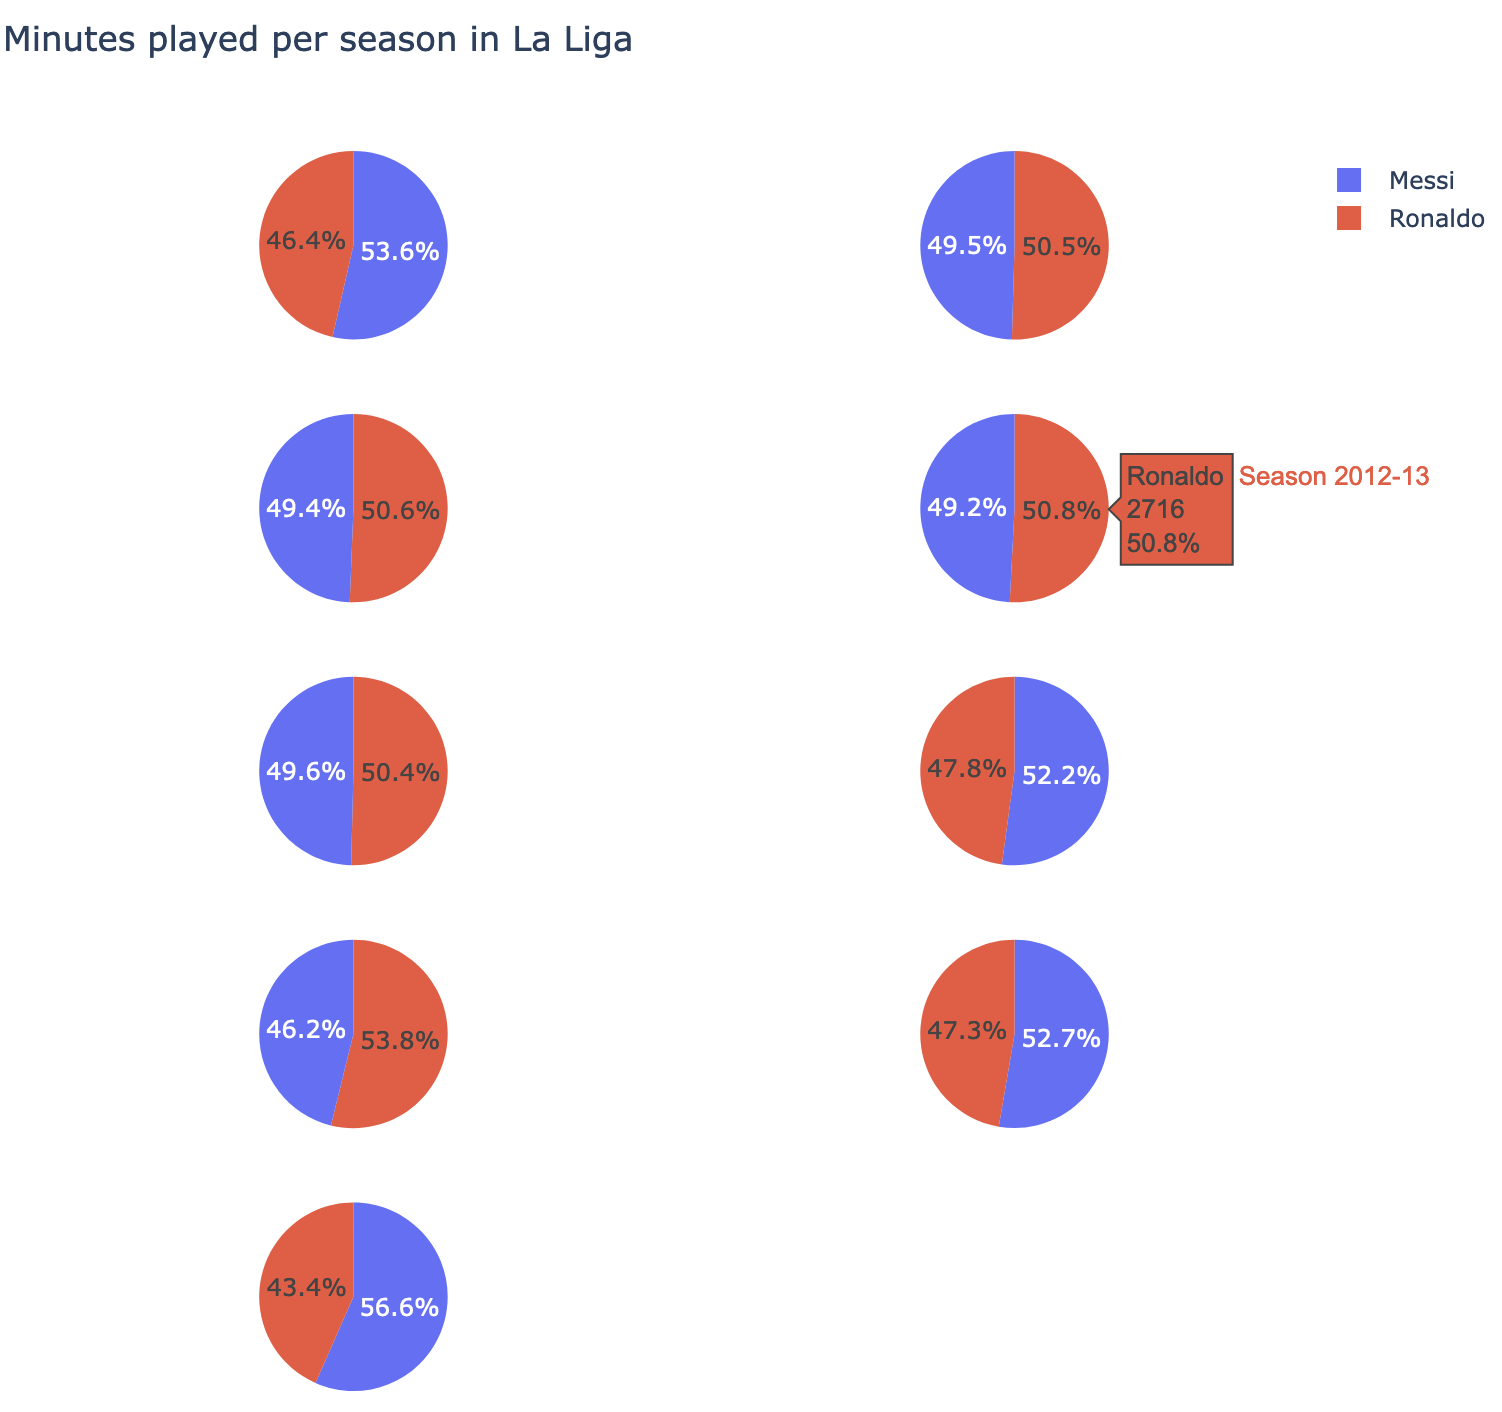
\includegraphics[width=7cm]{minutes_liga} }}%
        \qquad
        \subfloat[\centering Minutes played per season in Champions League]{{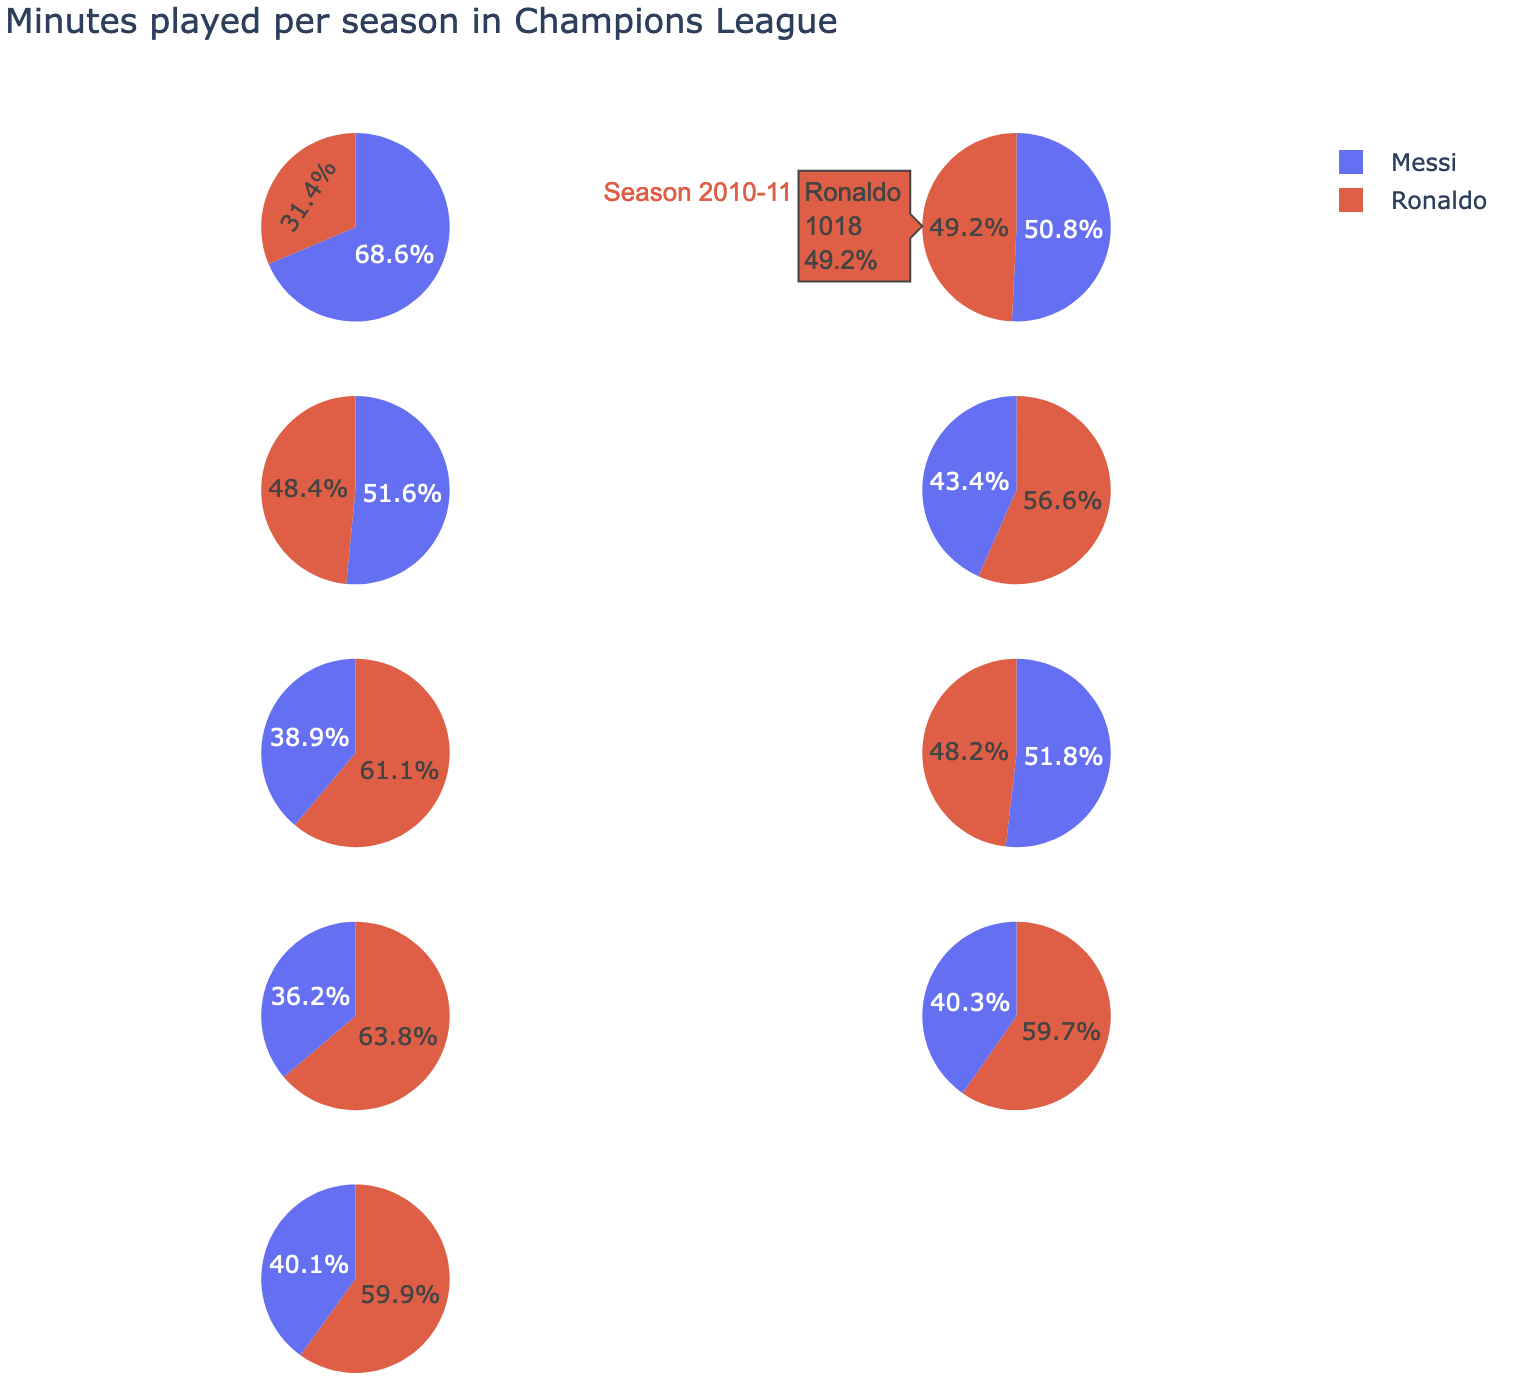
\includegraphics[width=7cm]{minutes_cl} }}%
        \caption{Minutes played per season}
        \label{fig:minutes}
    \end{figure}
    \item From the visualization, it's clear that the focus of Ronaldo shifted from la Liga to the Champions League towards the last few seasons, whereas Messi aimed to balance his time between both competetions more evenly.
    \item For the visual encoding, we use the following:
    \begin{itemize}
        \item Chart type used is a \textbf{Pie Chart}  
        \item We use colors as a \textbf{Channel}, with Red signifying statistics for Ronaldo and Blue for Messi.  
        \item We also use a \textbf{Ordering Direction} from left to right, with the left topmost pie chart being the statistics for the very first season i.e the 2009-10 season.  
    \end{itemize}
\end{itemize}
\subsubsection{Player form over all seasons}
\begin{itemize}
    \item Here, we aim to analyze the player form over all seasons. To determine the player form, we use a crude metric of number of goals scored per minute in each competetiion.
    \begin{figure}[H]
        \centering
        \subfloat[\centering Form per season in La Liga]{{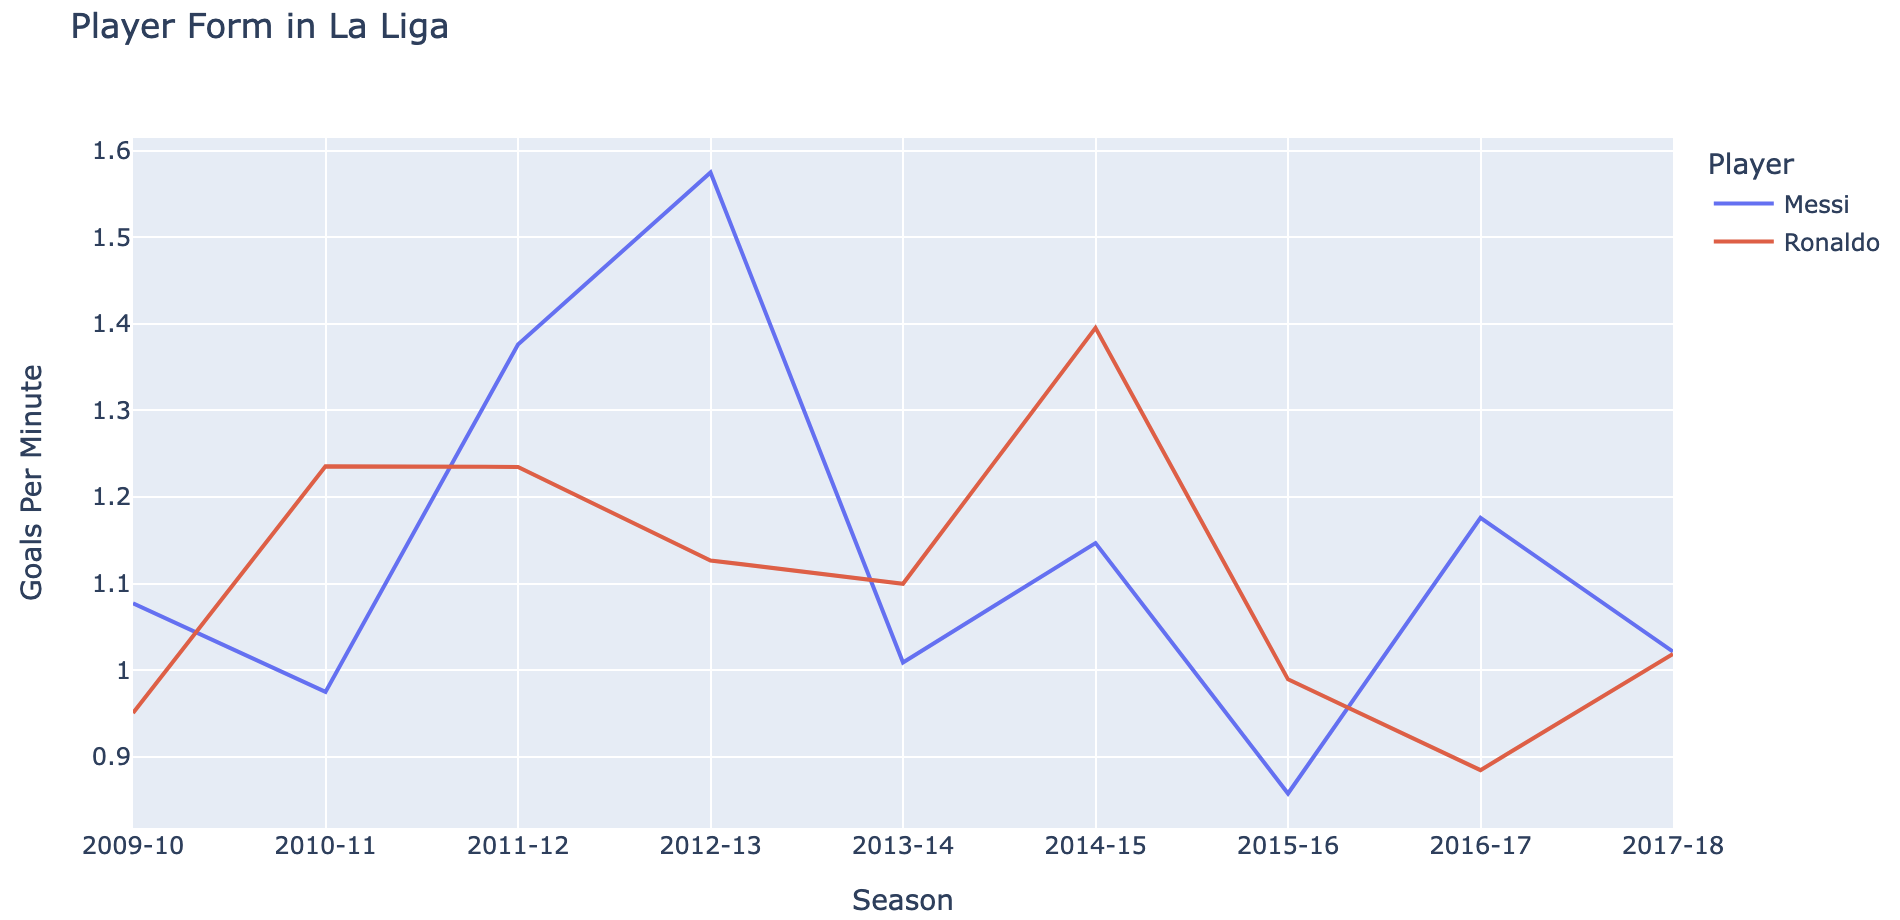
\includegraphics[width=8cm]{form_liga} }}
        \qquad
        \subfloat[\centering Form per season in Champions League]{{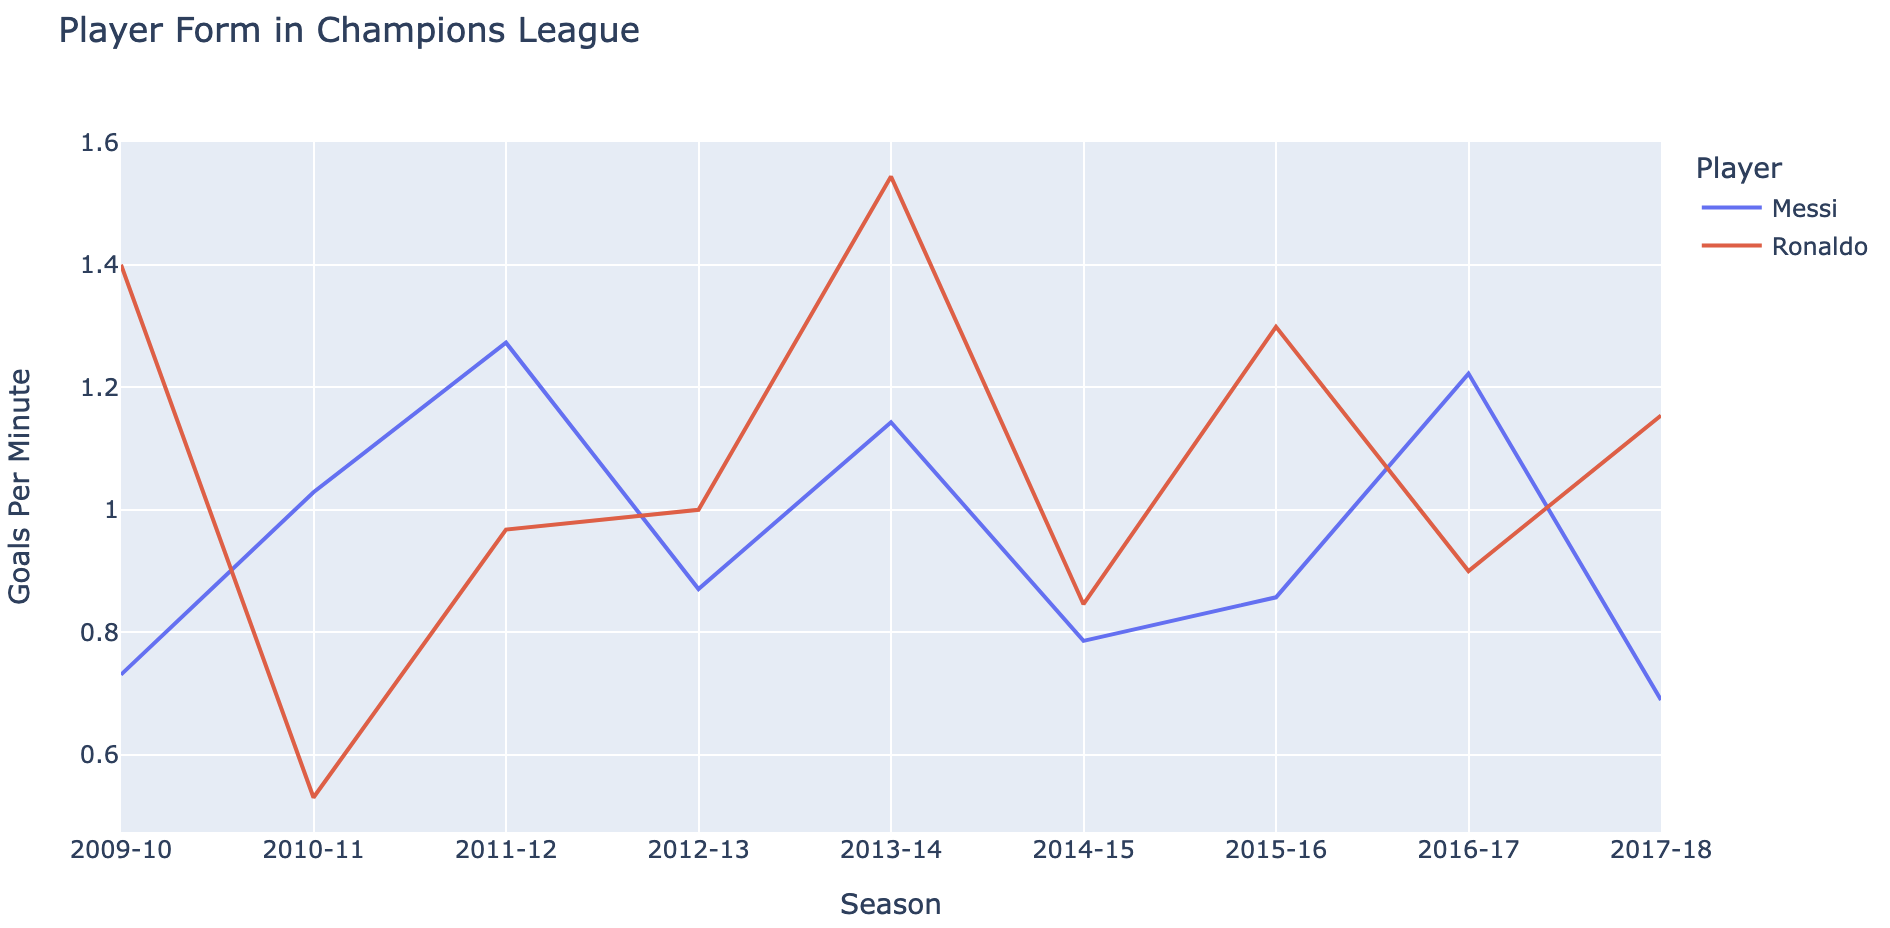
\includegraphics[width=8cm]{form_cl} }}
        \caption{Player Form per season}
        \label{fig:form}
    \end{figure}
    \item From the visualization, it's clear that Messi was dominant in La Liga during the 2011-12 and 2012-13 season, in which he scored a record 91 Goals. We can also see that in the same time, Ronaldo was more dominant in the Champions League, averaging almost 1.6 goals per minute!
    \item For the visual encoding, we use the following:
    \begin{itemize}
        \item Chart type used is a \textbf{Timeseries based Line Chart}  
        \item The x-axis contains the season, which is a string variable.
        \item The y-axis contains the average number of goals per minute, which is a quantitative variable.
        \item We use colors as a \textbf{Channel}, with Red signifying statistics for Ronaldo and Blue for Messi.  
    \end{itemize}
\end{itemize}
\subsection{Harry Potter Dataset: Statistical and Textual Visualizations}
\begin{itemize}
    \item Here, we aim to analyze the Harry potter dataset, and focus on creating both statistical and text based visualizations.
\end{itemize}
\subsubsection{Running time of each movie?}
\begin{itemize}
    \item We aim to visualize the running time of each movie in a simple plot.
    \begin{figure}[H]
        \centering
        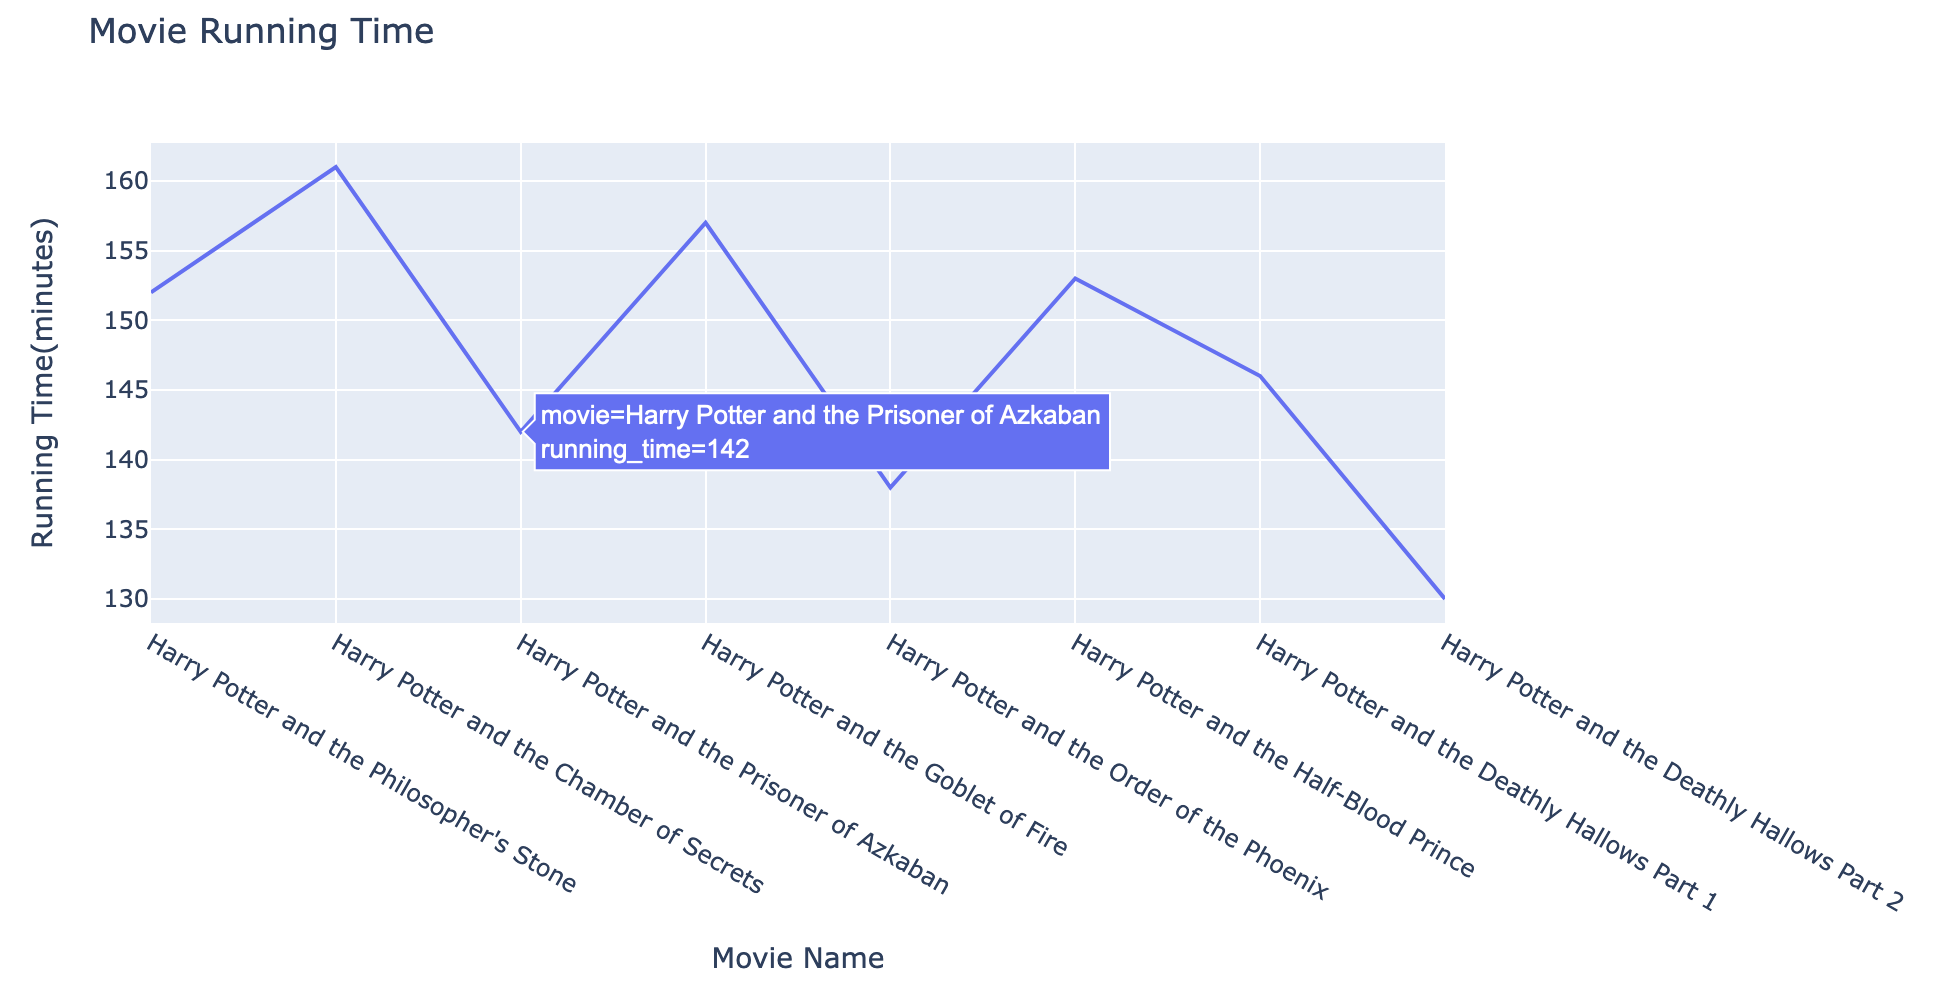
\includegraphics[width=0.8\textwidth]{running_time}
        \caption{Running time for each movie}
        \label{fig:running_time}
    \end{figure}
    \item From the above figure, we can see that while the first few movies focussed on having a high running time, the movies have grown shorter as time has passed, possibly to account for shorter attention spans!
    \item For the visual encoding, we use the following:
    \begin{itemize}
        \item The chart type used in a \textbf{Line Chart}  
        \item The x-axis contains the name of the movie, which is a string/categorical variable.
        \item The y-axis contains the total running time of the movie, which is a quantitative variable, in minutes.
    \end{itemize}
\end{itemize}
\subsubsection{Budget vs Box Office collection}
\begin{itemize}
    \item We aim to visualize the budget vs box office collection, as an indicator of how popular a given harry potter movie was during the time it was released.
    \begin{figure}[H]
        \centering
        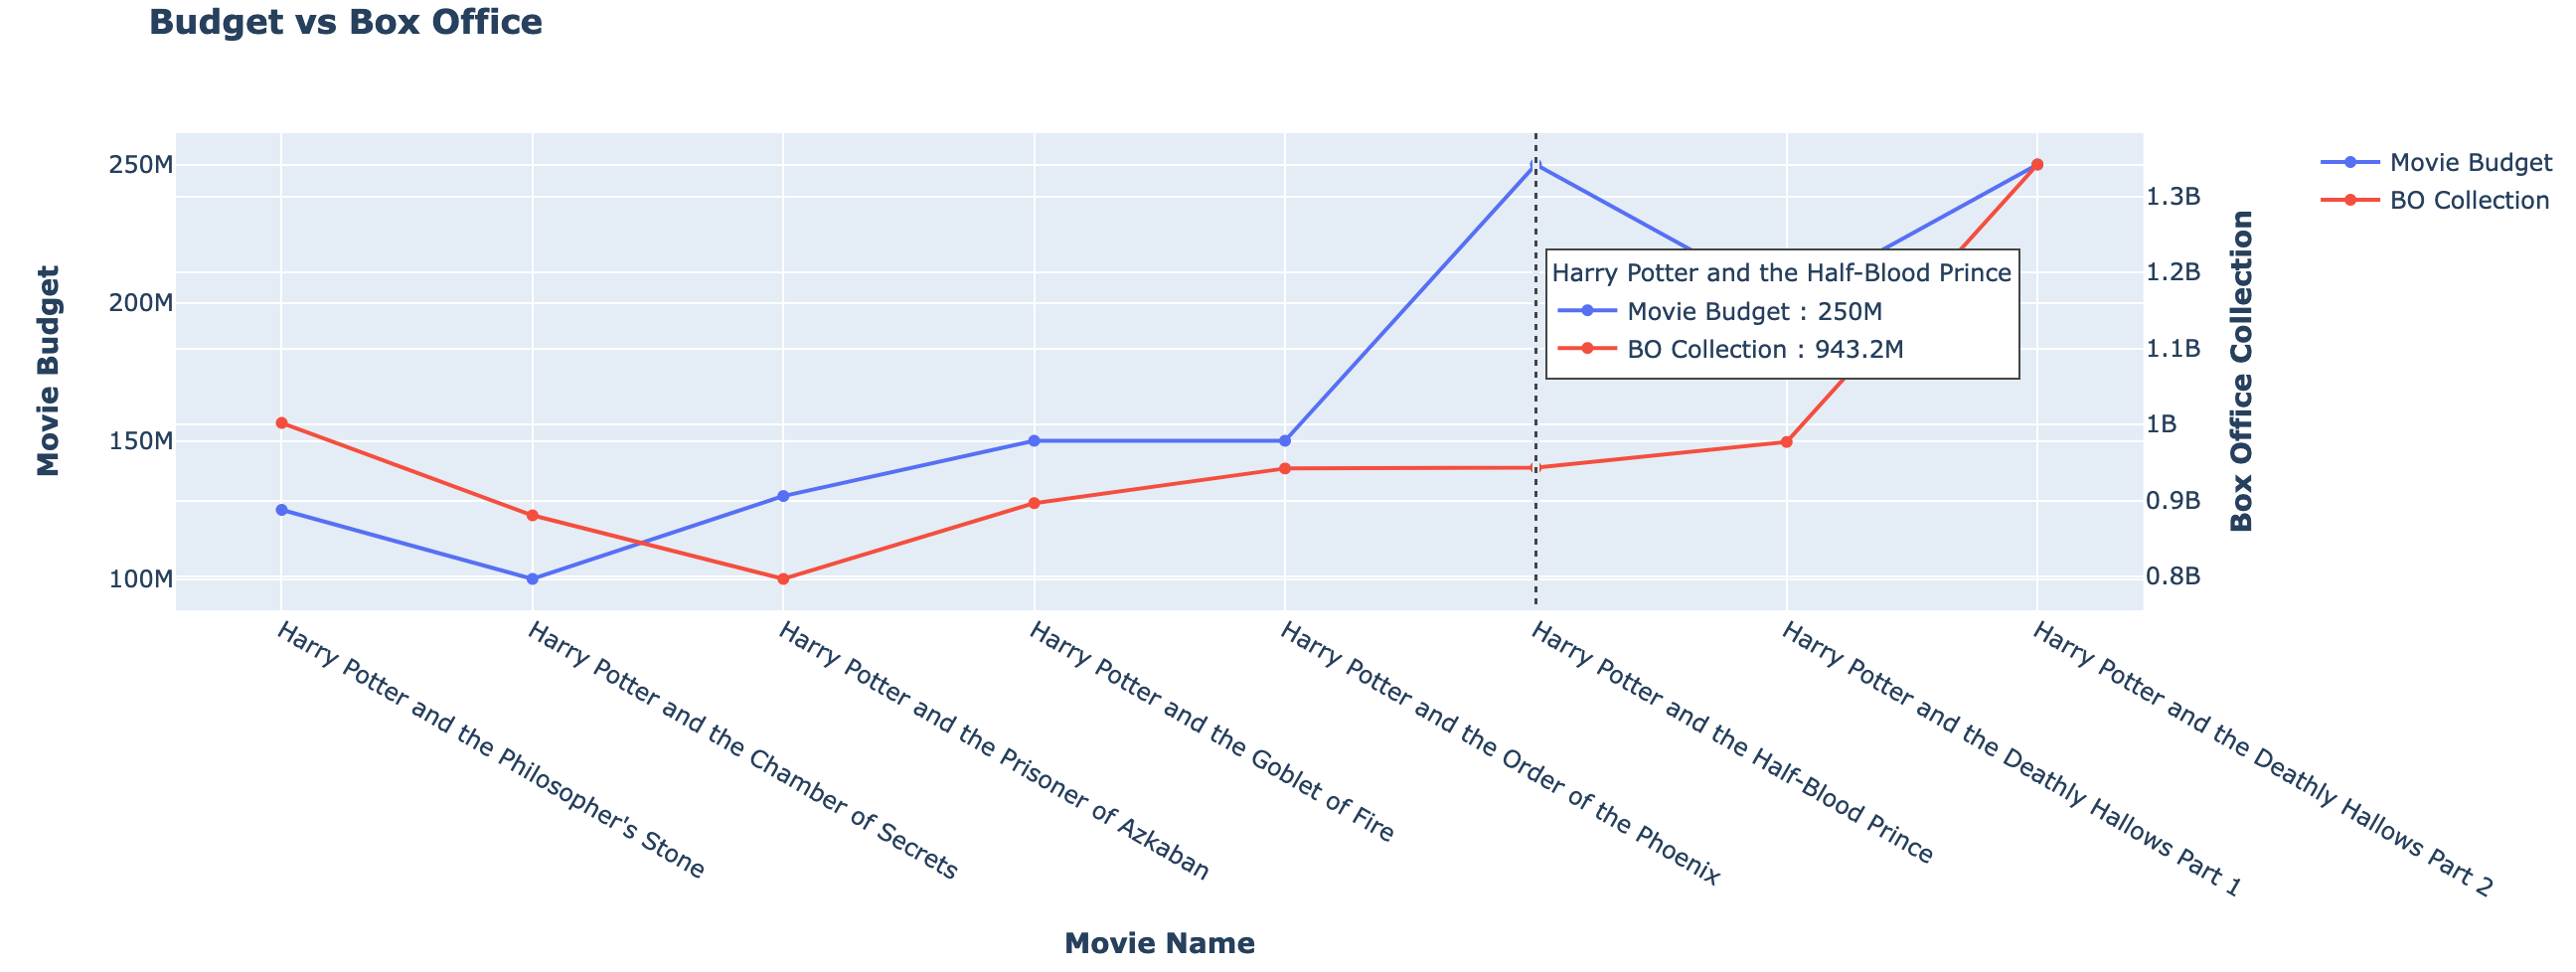
\includegraphics[width=0.8\textwidth]{box_office}
        \caption{Budget vs Box Office Collection for each movie}
        \label{fig:box_office}
    \end{figure}
    \item From the visualization, we see that only the first and the last harry potter movies had a collection of more than 1 Billion Dollars!
    \item The visual encoding used is as follows:
    \begin{itemize}
        \item The chart type used in a \textbf{Line Chart with Dual axis}  
        \item The x-axis contains the name of the movie, which is a string/categorical variable.
        \item The y-axis on the left, is a quantitative variable, and contains the budget of the movie. The scale is in millions
        \item The y-axis on the right, is a quantitative variable, and contains the box office collection of the movie. The scale is in Billions.
        \item We also use color as \textbf{Channels}, with blue depicting the movie budget and red depicting the Box office collection.  
    \end{itemize}
\end{itemize}
\subsubsection{Who had the most number of dialogues?}
\begin{itemize}
    \item Here, we aim to determine which character had the most number of dialogues, across all movies.
    \begin{figure}[H]
        \centering
        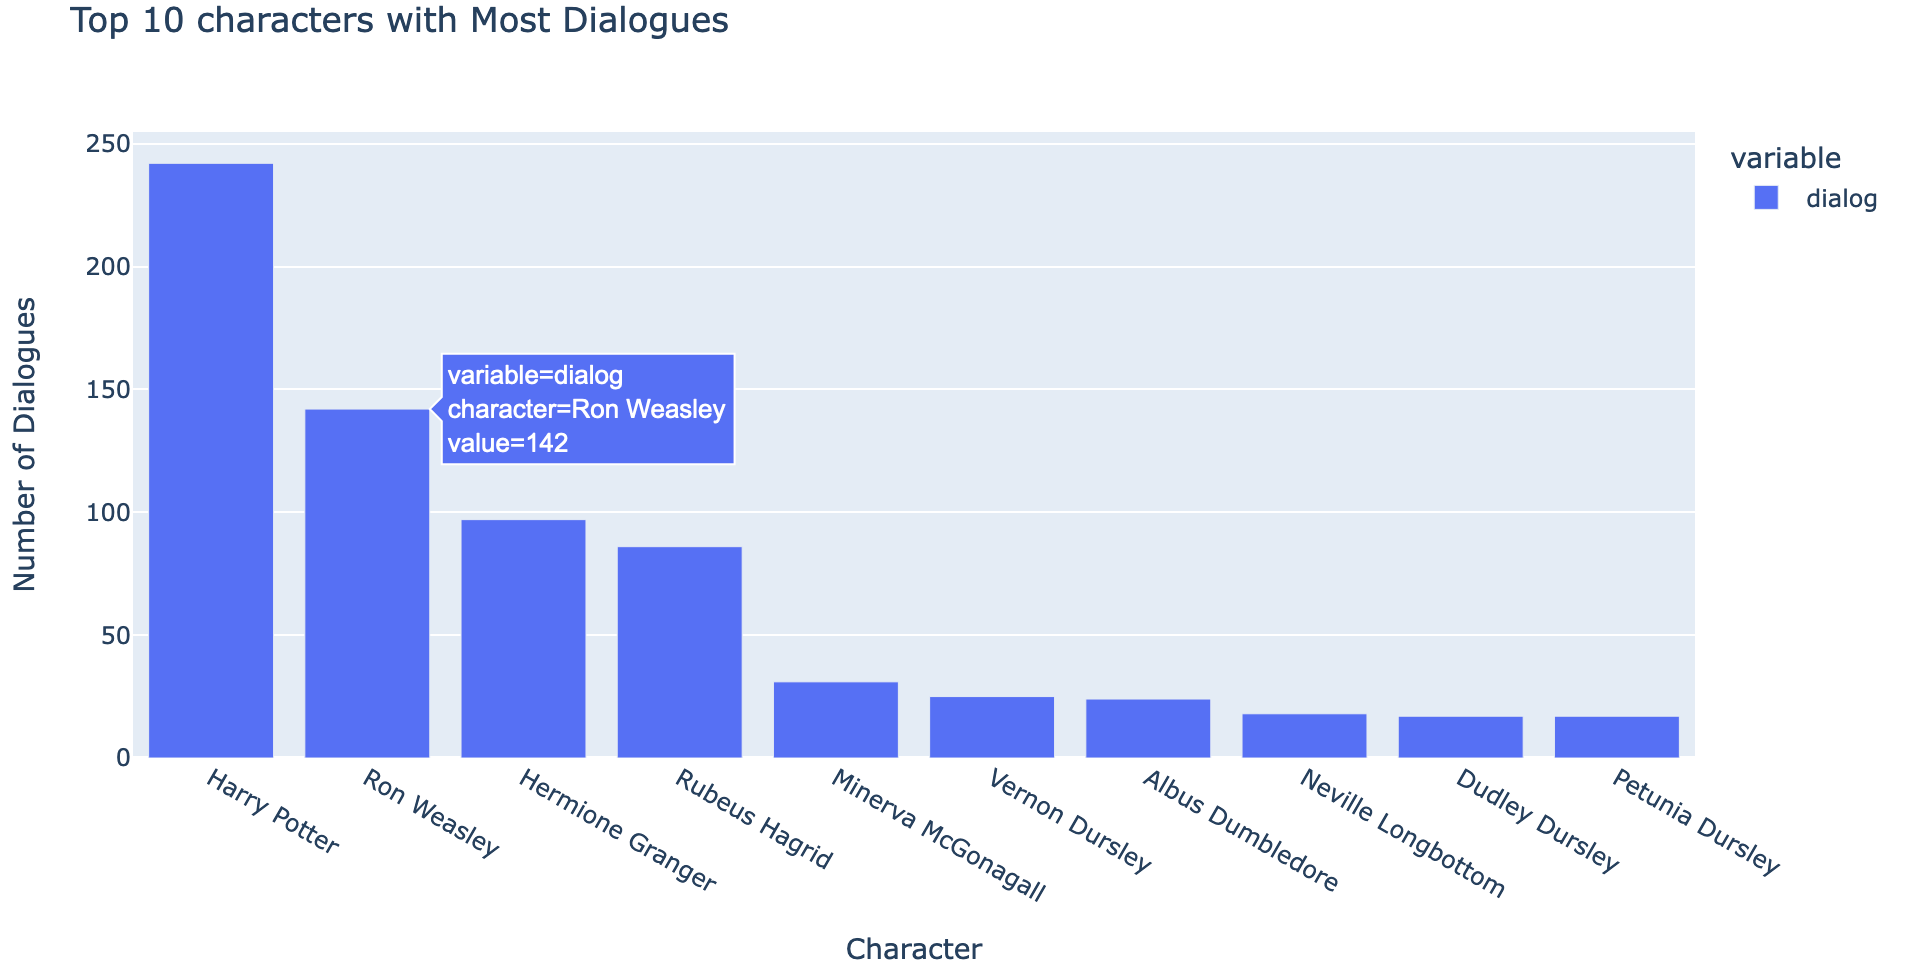
\includegraphics[width=0.6\textwidth]{dialog}
        \caption{Top 10 characters with most dialogues}
        \label{fig:dialog}
    \end{figure}
    \item We see that the main protagonists had the most amount of dialogues, followed by their supporting characters/mentors such as Hagrid, Dumbledore, etc.
    \item The visual encoding used is as follows:
    \begin{itemize}
        \item The chart type used is a \textbf{Bar Chart}  
        \item The x-axis is a string/categorical variable, and denotes the name of the character.
        \item The y-axis is a quantitative variable, and denotes the number of dialogues spoken by a given character across all movies
    \end{itemize}
\end{itemize}
\subsubsection{Word Cloud of Dialogues}
\begin{itemize}
    \item Here, we aim to visualize the dialogues spoken by Harry Potter in all movies.
    \item For preprocessing, we lowercase all the given words, and remove the stopwords.
    \item We create a contour mask using a harry potter stencil image, which gives the visualization the shape of the actor.
    \item Finally, we only display the top 2000 words.
    \begin{figure}[H]
        \centering
        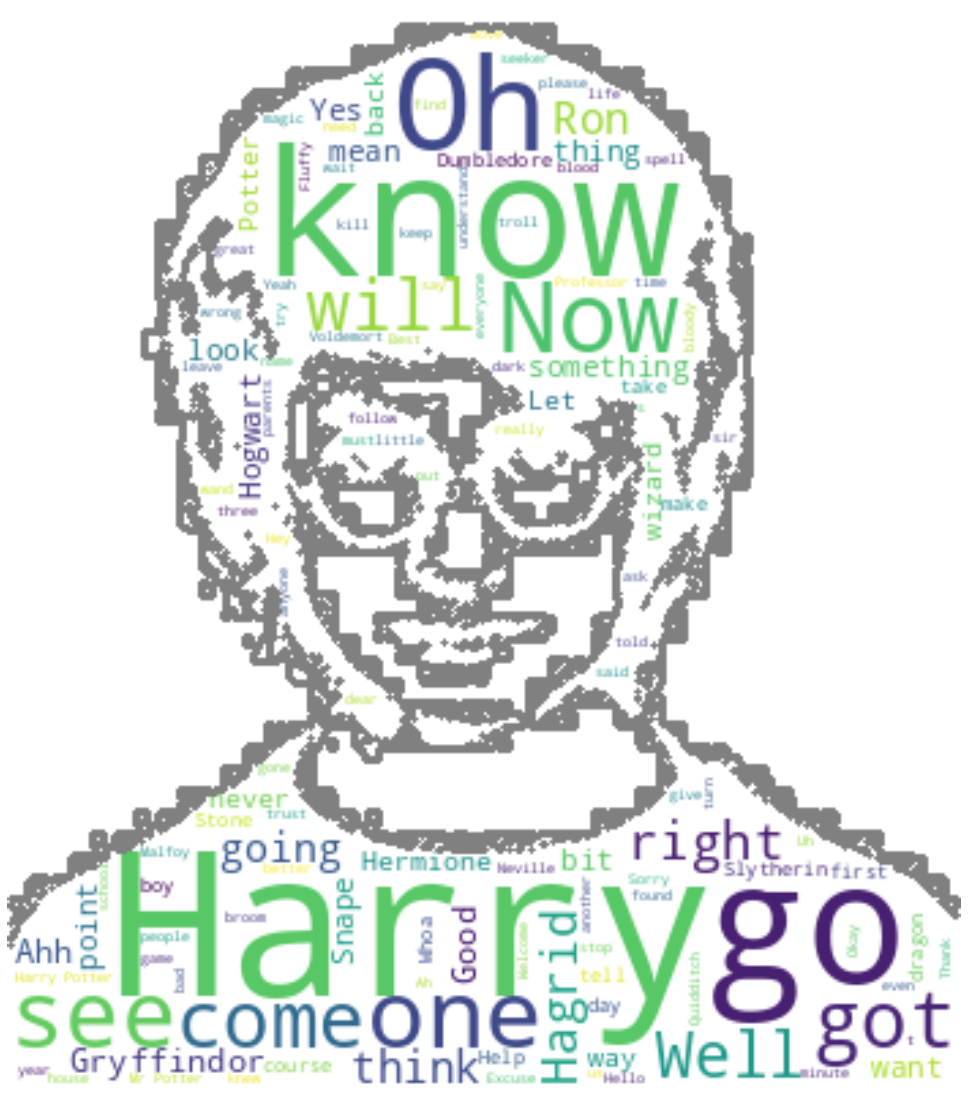
\includegraphics[width=0.2\textwidth]{wordcloud}
        \caption{Wordcloud of Harry Potter Dialogues}
        \label{fig:wordcloud}
    \end{figure}
    \item From the above visualization, it's clear that:
    \begin{itemize}
        \item As expected, "Harry" is the most common word.
        \item Apart from mentions of other characters, we also see mentions of the different in the movie, such as Gryffindor(the house to which Harry was assigned) and Slytherin(The house which Harry was praying was not assigned to him!)
    \end{itemize}
    \item The chart type is \textbf{Wordcloud}. Size of the word is used as \textbf{Channel} to denote how many times the word was spoken by the character.  
\end{itemize}
\subsubsection{Distribution of words spoken by a character.}
\begin{itemize}
    \item We aim to visualize the different sequence of words using a wordtree.
    \item Here, we analyze the dialogues of Dumbledore, but focus on the word "Potter" i.e the instances where he has mentioned potter.
    \begin{figure}[H]
        \centering
        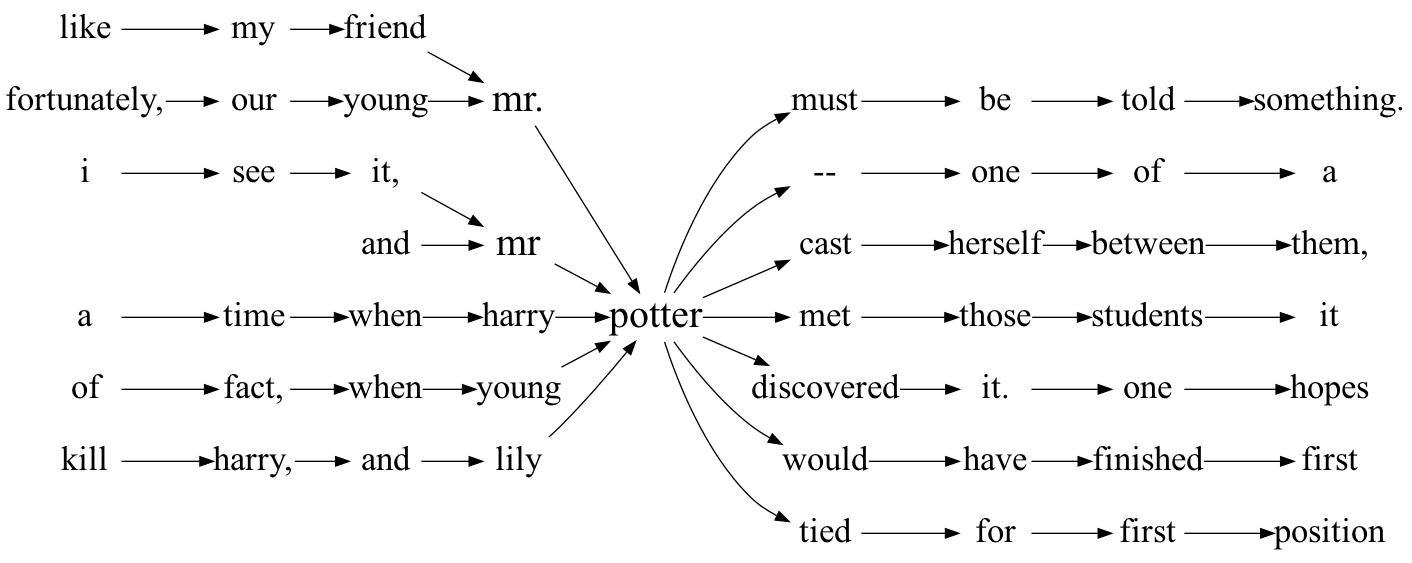
\includegraphics[width=0.6\textwidth]{potter.gv}
        \caption{Wordtree of Dumbledore Dialogues for the word Potter}
        \label{fig:potter}
    \end{figure}
    \item The chart type used is a \textbf{Double Wordtree}  
\end{itemize}
\subsubsection{Topic Detection}
\begin{itemize}
    \item Here, we aim to visualize the main topics present in the dialogues by Harry Potter.
    \item For preprocessing the data, we convert all words to lowercase and filter words with alphabets that are atleast 3 letters long.
    \item We also remove the stopwords to reduce the noise in the topics.
    \item For creating the vectors, we use Term Frequence - Inverse Document Frequency(TF-IDF)
    \item Finally, we detect the topics using the Latent Dirchlet Algorithm(LDA).
    \begin{figure}[H]
        \centering
        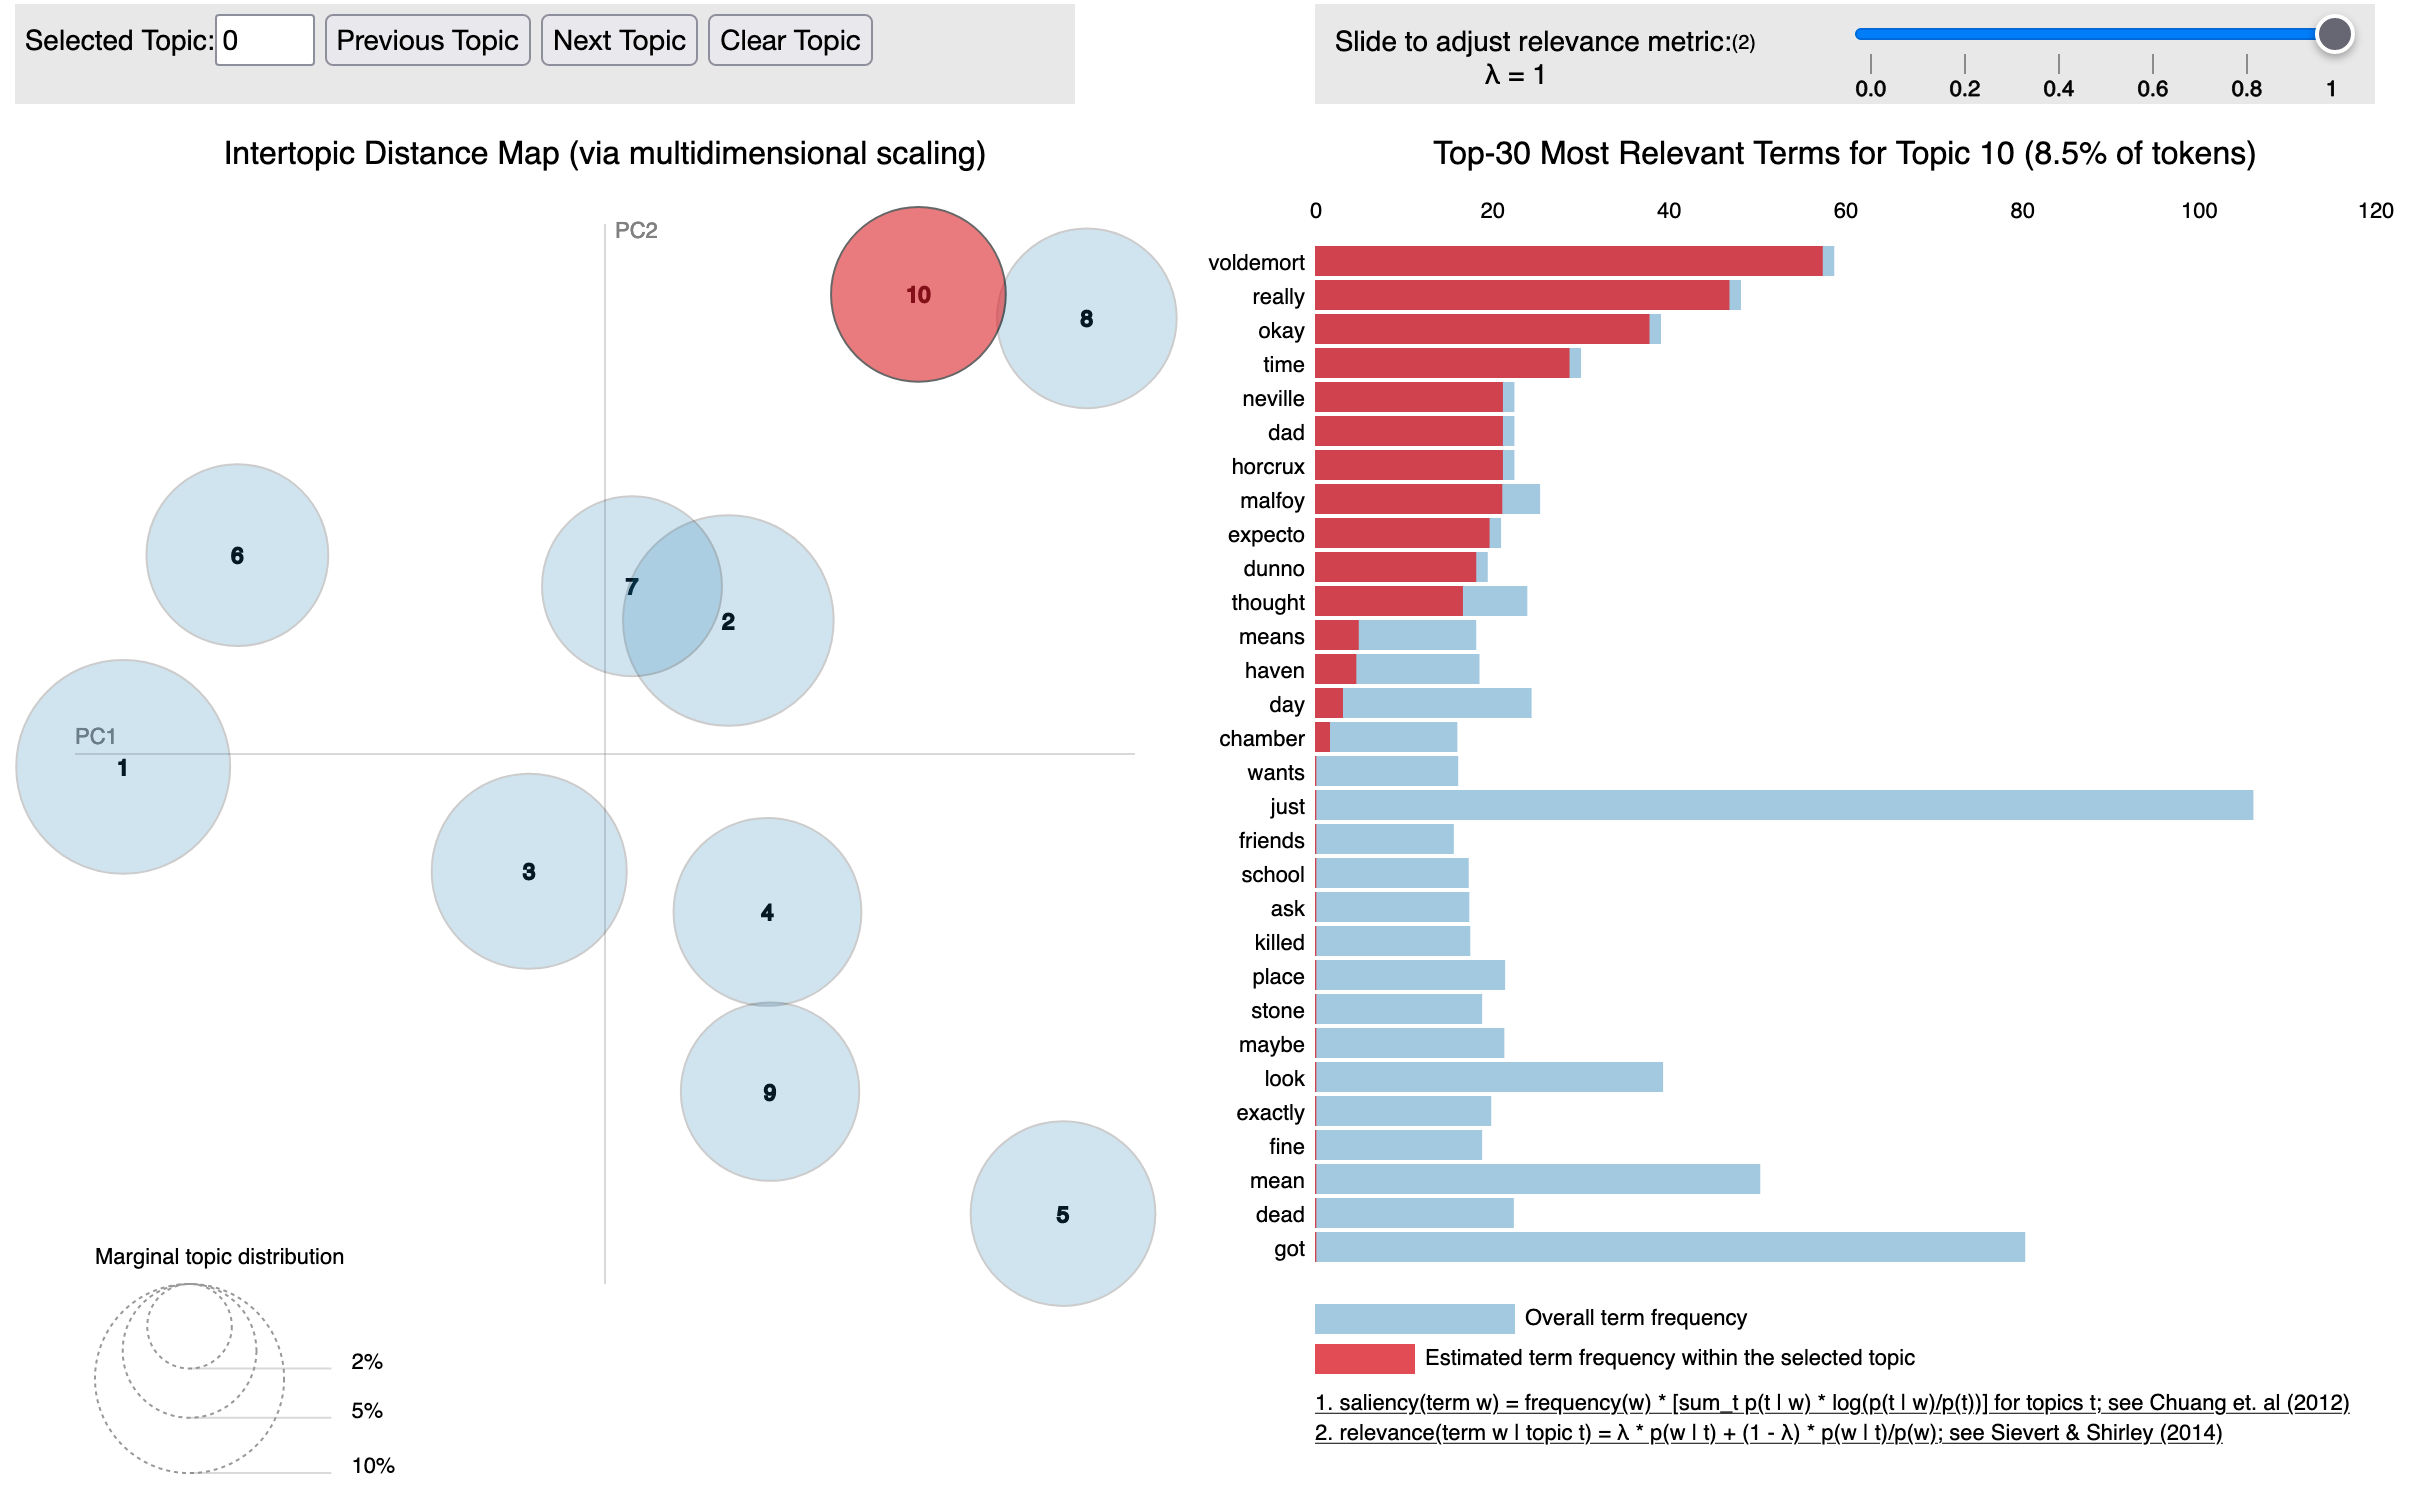
\includegraphics[width=0.4\textwidth]{topic}
        \caption{Topic Modelling using LDA on dialogues by Harry Potter}
        \label{fig:topic}
    \end{figure}
    \item From the above visualization, we see that:
    \begin{itemize}
        \item We experiment with different number of topics, and obtained the best results when the number of topics is 10.
        \item There are other topics dedicated to specific characters such as:
        \begin{itemize}
            \item Topic number 10 is specifically for voldermort and horcuxes, which are a source of his power!
            \item Topic number 8 primarily contains dialogues about Ron.
            \item Topic number 6 primarily contains dialogues about Hermione.
        \end{itemize}
        \item We also see that, while topic number 1 is the largest, the words in this topic are general and don't point to anything specific. This could be considered as a "noisy" topic.
    \end{itemize}
    \item This visualization is a \textbf{Meso Level} visualization, since it focus on only the dialogues of Harry Potter. 
    \item We use circles as \textbf{Mark} to show the words in each cluster, and the size of the circle as \textbf{Channels}, to determine the number of words in the cluster. Large cluster contains more number of words.   
    \item Finally, on the right, we use a \textbf{Bar Chart} to display the total number of occurences of each word in the given topic. 
\end{itemize}
\section{References}
\begin{itemize}
    \item \href{https://towardsdatascience.com/end-to-end-topic-modeling-in-python-latent-dirichlet-allocation-lda-35ce4ed6b3e0}{Topic Modelling using LDA} 
    \item \href{https://www.betterevaluation.org/en/evaluation-options/wordtree}{Introduction to Wordtrees} 
    \item \href{https://www.analyticsvidhya.com/blog/2021/05/how-to-build-word-cloud-in-python/}{Wordcloud in Python}
\end{itemize}
\end{document}
